% Chapter 7, Section 4

\section{Dropout \difficultyInline{intermediate}}
\label{sec:dropout}

\textbf{Dropout} randomly deactivates neurons during training, preventing co-adaptation.

\subsection{Intuition: Training a Robust Ensemble}

Dropout is like asking different subsets of a team to work on the same task on different days. No single member can rely on a particular colleague always being present, so each learns to be broadly useful. This results in a robust team (model) that performs well even when some members (neurons) are inactive.

\subsection{Training with Dropout}

Training with dropout involves sampling a binary mask $\vect{m}$ with $P(m_i = 1) = p$ for each layer at each training step, then applying the mask to the activations: $\vect{h} = \vect{m} \odot \vect{h}$. Mathematically, this is expressed as $\vect{h}_{\text{dropout}} = \vect{m} \odot f(\mat{W}\vect{x} + \vect{b})$ where $m_i \sim \text{Bernoulli}(p)$, effectively randomly deactivating neurons with probability $1-p$ during training to prevent co-adaptation and improve generalization.

\begin{figure}[htbp]
\centering
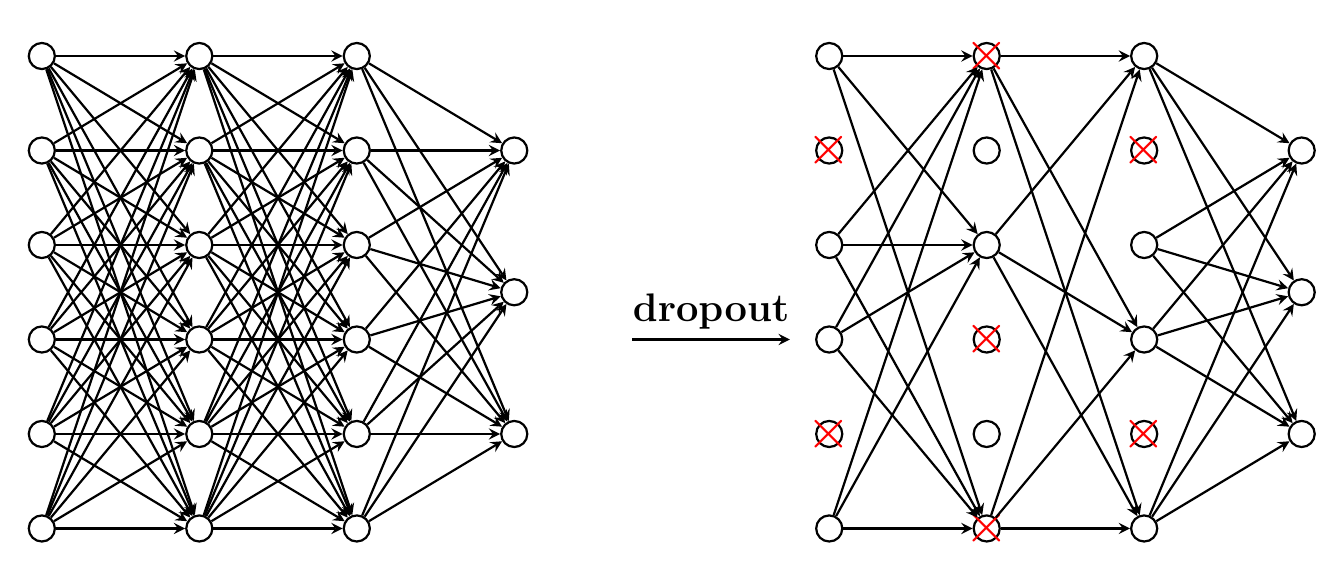
\begin{tikzpicture}[
    node/.style={circle, draw, thick},
  ]

\def\layersep{2}
\def\nodesep{1.2}

  % Input layer (6 nodes)
  \foreach \y in {1,...,6}{
      \node[node] (i\y) at (0,\nodesep*\y) {};
    }

  % Hidden layer 1 (6 nodes)
  \foreach \y in {1,...,6}{
      \node[node] (h1\y) at (\layersep,\nodesep*\y) {};
    }

  % Hidden layer 2 (6 nodes)
  \foreach \y in {1,...,6}{
      \node[node] (h2\y) at (2*\layersep,\nodesep*\y) {};
    }

  % Output layer (3 nodes)
  \node[node] (o1) at (3*\layersep,\nodesep*2) {};
  \node[node] (o2) at (3*\layersep,\nodesep*3.5) {};
  \node[node] (o3) at (3*\layersep,\nodesep*5) {};

  % Connections
  \foreach \source in {1,...,6}
  \foreach \dest in {1,...,6}{
      \path[-stealth, thick] (i\source) edge (h1\dest);
      \path[-stealth, thick] (h1\source) edge (h2\dest);
    }
  \foreach \source in {1,...,6}
  \foreach \dest in {1,2,3}
  \draw[-stealth, thick] (h2\source) -- (o\dest);

  % Dropout arrow
  \draw[-stealth, thick] (7.5,3*\nodesep) -- node[above,font=\Large\bfseries] {dropout} (9.5, 3*\nodesep);

  % After dropout - Input layer (6 nodes, drop 2)
  \foreach \y in {1,...,6}
  \node[node] (di\y) at (10,\nodesep*\y) {};

  \node[red,font=\huge] at (di2) {$\times$};
  \node[red,font=\huge] at (di5) {$\times$};

  % After dropout - Hidden layer 1 (6 nodes, drop 3)
  \foreach \y in {1,...,6}
  \node[node] (dh1\y) at (10+\layersep,\nodesep*\y) {};

  \node[red,font=\huge] at (dh11) {$\times$};
  \node[red,font=\huge] at (dh13) {$\times$};
  \node[red,font=\huge] at (dh16) {$\times$};

  % After dropout - Hidden layer 2 (6 nodes, drop 2)
  \foreach \y in {1,...,6}
  \node[node] (dh2\y) at (10+2*\layersep,\nodesep*\y) {};

  \node[red,font=\huge] at (dh22) {$\times$};
  \node[red,font=\huge] at (dh25) {$\times$};

  % After dropout - Output layer (3 nodes)
  \node[node] (do1) at (10+3*\layersep,\nodesep*2) {};
  \node[node] (do2) at (10+3*\layersep,\nodesep*3.5) {};
  \node[node] (do3) at (10+3*\layersep,\nodesep*5) {};

  % After dropout connections
  \foreach \source in {1,3,4,6}
  \foreach \dest in {1,4,6}
  \draw[-stealth, thick] (di\source) -- (dh1\dest);

  \foreach \source in {1,4,6}
  \foreach \dest in {1,3,6}
  \draw[-stealth, thick] (dh1\source) -- (dh2\dest);

  \foreach \source in {1,3,4,6}
  \foreach \dest in {1,2,3}
  \draw[-stealth, thick] (dh2\source) -- (do\dest);

\end{tikzpicture}
\caption{Dropout training: randomly deactivating neurons ($\times$) creates subnetworks, forcing robustness.}
\label{fig:dropout-training-process}
\end{figure}

\subsection{Inference}

At test time, scale outputs by dropout probability:
\begin{equation}
\vect{h}_{\text{test}} = p \cdot f(\mat{W}\vect{x} + \vect{b})
\end{equation}

Or equivalently, scale weights during training by $\frac{1}{p}$ (inverted dropout).

In practice, modern frameworks implement \emph{inverted dropout}: during training, activations are scaled by $\tfrac{1}{p}$ after masking so that the expected activation matches test-time activations, and no scaling is needed at inference \cite{Srivastava2014,GoodfellowEtAl2016}. For convolutional layers, use the same $p$ per feature map to avoid distribution shift.

\subsection{Interpretation}

Dropout can be viewed as an implicit ensemble where sampling masks trains an ensemble of $2^n$ subnetworks whose shared weights yield a form of model averaging. It also acts as noise injection where multiplicative Bernoulli noise on activations provides data-dependent regularization analogous to adding Gaussian noise for linear models. Additionally, dropout relates to approximate Bayesian inference where with appropriate priors, it connects to variational inference, and applying dropout at test time with multiple passes (MC dropout) estimates predictive uncertainty, making it useful for uncertainty quantification in safety-critical applications.

\begin{example}
\textbf{Example (uncertainty):} Run $T=20$ stochastic forward passes with dropout enabled at test time and average predictions to obtain mean and variance; high variance flags low-confidence inputs.
\end{example}

\subsection{Variants}

DropConnect drops individual weights instead of activations, promoting sparsity at the parameter level and providing a different form of regularization. Spatial Dropout drops entire feature maps in CNNs to preserve spatial coherence and regularize channel reliance, which is particularly useful for convolutional layers. Variational Dropout uses the same dropout mask across time steps in RNNs to avoid injecting different noise per step that can harm temporal consistency, making it more suitable for sequential data. MC Dropout keeps dropout active at inference and averages predictions to quantify epistemic uncertainty, which is useful in safety-critical applications where uncertainty estimation is crucial. Concrete and Alpha Dropout provide continuous relaxations or distributions tailored for specific activations like SELU to maintain self-normalizing properties, offering more sophisticated regularization approaches for specific network architectures.

\begin{figure}[htbp]
\centering
\begin{tikzpicture}[scale=0.9]
    % simple schematic: three subnetworks averaged
    \node[draw, rectangle, fill=bookpurple!15] (s1) at (0,0) {Subnetwork 1};
    \node[draw, rectangle, fill=bookpurple!15] (s2) at (3,0) {Subnetwork 2};
    \node[draw, rectangle, fill=bookpurple!15] (s3) at (6,0) {Subnetwork 3};
    \node[draw, circle, fill=bookpurple!20] (avg) at (3,-1.8) {Average};
    \draw[->] (s1) -- (avg);
    \draw[->] (s2) -- (avg);
    \draw[->] (s3) -- (avg);
\end{tikzpicture}
\caption{Dropout as implicit model averaging over many subnetworks.}
\label{fig:dropout-ensemble}
\end{figure}

\begin{figure}[htbp]
\centering
\begin{tikzpicture}[scale=0.9]
    % Layer nodes
    \foreach \i in {1,2,3}
        \node[circle, draw, fill=bookpurple!15, minimum size=0.7cm] (x\i) at (0,-\i) {};
    \foreach \i in {1,2,3,4}
        \node[circle, draw, fill=bookpurple!25, minimum size=0.7cm] (h\i) at (2,-\i*0.8) {};
    \foreach \i in {1,2}
        \node[circle, draw, fill=bookred!15, minimum size=0.7cm] (y\i) at (4,-\i) {};

    % Full connections (light color)
    \foreach \i in {1,2,3}
        \foreach \j in {1,2,3,4}
            \draw[->,bookpurple!30] (x\i) -- (h\j);
    \foreach \i in {1,2,3,4}
        \foreach \j in {1,2}
            \draw[->,bookpurple!30] (h\i) -- (y\j);

    % Dropped neurons (crossed)
    \draw[bookred, line width=1.2pt] (h2) ++(-0.25,-0.25) -- ++(0.5,0.5);
    \draw[bookred, line width=1.2pt] (h2) ++(0.25,-0.25) -- ++(-0.5,0.5);
    \draw[bookred, line width=1.2pt] (h4) ++(-0.25,-0.25) -- ++(0.5,0.5);
    \draw[bookred, line width=1.2pt] (h4) ++(0.25,-0.25) -- ++(-0.5,0.5);

    \node at (2,0.5) {\small Randomly dropped (training)};
\end{tikzpicture}
\caption{Dropout during training: randomly deactivating hidden units encourages redundancy.}
\label{fig:dropout-diagram}
\end{figure}

% Index entries
\index{dropout}
\index{regularization!dropout}

